\documentclass[a4paper,14pt]{extreport}
  \usepackage[left=1.5cm,right=1.5cm,
      top=1.5cm,bottom=2cm,bindingoffset=0cm]{geometry}
  \usepackage{scrextend}
  \usepackage[T1,T2A]{fontenc}
  \usepackage[utf8]{inputenc}
  \usepackage[english,russian,ukrainian]{babel}
  \usepackage{tabularx}
  \linespread{1.3}
  \usepackage[colorinlistoftodos]{todonotes}
  \usepackage{amssymb}
  \usepackage{color}
  \usepackage{amsmath}
  \usepackage{mathrsfs}
  \usepackage{listings}
  \usepackage{graphicx}
  \graphicspath{ {./images/} }
  \usepackage{lipsum}
  \usepackage{xcolor}
  \usepackage{hyperref}
  \usepackage{tcolorbox}

  \usepackage[framemethod=TikZ]{mdframed}
  \usepackage{wrapfig,boxedminipage,lipsum}
  \mdfdefinestyle{MyFrame}{%
  linecolor=blue,outerlinewidth=2pt,roundcorner=20pt,innertopmargin=\baselineskip,innerbottommargin=\baselineskip,innerrightmargin=20pt ,innerleftmargin=20pt,backgroundcolor=gray!50!white}
   \usepackage{csvsimple}
   \usepackage{supertabular}
  \usepackage{pdflscape}
  \usepackage{fancyvrb}
  %\usepackage{comment}
  \usepackage{array,tabularx}
  \usepackage{colortbl}

  \usepackage{varwidth}
  \tcbuselibrary{skins}
  \usepackage{fancybox}
  \usepackage{spreadtab}


  \usepackage{tikz}
  \usepackage[framemethod=TikZ]{mdframed}
  \usepackage{xcolor}
  \usetikzlibrary{calc}
  \makeatletter
  \newlength{\mylength}
  \xdef\CircleFactor{1.1}
  \setlength\mylength{\dimexpr\f@size pt}
  \newsavebox{\mybox}
  \newcommand*\circled[2][draw=blue]{\savebox\mybox{\vbox{\vphantom{WL1/}#1}}\setlength\mylength{\dimexpr\CircleFactor\dimexpr\ht\mybox+\dp\mybox\relax\relax}\tikzset{mystyle/.style={circle,#1,minimum height={\mylength}}}
  \tikz[baseline=(char.base)]
  \node[mystyle] (char) {#2};}
  \makeatother
   % Цвета для гиперссылок
  \definecolor{linkcolor}{rgb}{0, 0.72, 0.92} % цвет ссылок
  \definecolor{urlcolor}{rgb}{0.0, 0.0, 1.0}% цвет гиперссылок
  \hypersetup{pdfstartview=FitH,  linkcolor=black,urlcolor=black,citecolor=red, colorlinks=true}

  \definecolor{ggreen}{rgb}{0.4,1,0}
  \definecolor{rred}{rgb}{1,0.1,0.1}
  \definecolor{amber}{rgb}{1.0, 0.75, 0.0}
  \definecolor{babyblue}{rgb}{0.54, 0.81, 0.94}
  \definecolor{amethyst}{rgb}{0.6, 0.4, 0.8}

  \usepackage{float}
  \usepackage{wrapfig}
  \usepackage{framed}
  %for nice Code{
  \lstdefinestyle{customc}{
    belowcaptionskip=1\baselineskip,
    breaklines=true,
    frame=L,
    xleftmargin=\parindent,
    language=C,
    showstringspaces=false,
    basicstyle=\small\ttfamily,
    keywordstyle=\bfseries\color{green!40!black},
    commentstyle=\itshape\color{purple!40!black},
    identifierstyle=\color{blue},
    stringstyle=\color{orange},
  }
  \lstset{escapechar=@,style=customc}
%}


\begin{document}
\renewcommand{\bibname}{Список використаної літератури}% -- переименуем название списка литературы


%указатель -- \cite{lit1}

\pagecolor{white}

%----------------------------------------1
\newtcbox{\xmybox}[1][red]{on line, arc=7pt,colback=#1!10!white,colframe=#1!50!black, before upper={\rule[-3pt]{0pt}{10pt}},boxrule=1pt, boxsep=0pt,left=6pt,right=6pt,top=2pt,bottom=2pt}

\begin{titlepage}
  \begin{center}
  \large
  Національний технічний університет України \\ "Київський політехнічний інститут імені Ігоря Сікорського"


  Факультет Електроніки

  Кафедра мікроелектроніки
  \vfill

  \textsc{РЕФЕРАТ}\\

  %{\Large Про виконання лабораторної роботи №1\\
  з дисципліни: «Функціональна електроніка»\\[1cm]

  Піроелектричні перетворювачі (ІЧ) зображення


  %}
  \bigskip
  \end{center}
  \vfill

  \newlength{\ML}
  \settowidth{\ML}{«\underline{\hspace{0.4cm}}» \underline{\hspace{2cm}}}
  \hfill
  \begin{minipage}{1\textwidth}
  Виконавець:\\
  Студент 4-го курсу \hspace{4cm} $\underset{\text{(підпис)}}{\underline{\hspace{0.2\textwidth}}}$  \hspace{1cm}Лищенко Б. В.\\
  \vspace{1cm}

  Перевірила: \hspace{5.6cm} $\underset{\text{(підпис)}}{\underline{\hspace{0.2\textwidth}}}$  \hspace{1cm}доц. Обухова Т. Ю.\\

  \end{minipage}

  \vfill

  \begin{center}
  2021
  \end{center}
\end{titlepage}
\tableofcontents
\setcounter{page}{2}

\newpage

\chapter{Вступ}\par
  Неохолоджувані теплові приймачі хоч і поступаються
фотонним і квантовим за своїми граничними параметрами, мають цілу низку характеристик, які роблять їх незамінними в великій області
застосувань. Це, зокрема, стосується завдань
спостереження та розпізнавання об'єктів на невеликих
відстанях (до 2500 м), ІЧ-мікроскопії, медичної та промислової діагностики тощо. Головне
перевага тепловізійних систем на багатоелементних теплових приймачах (UFPA) перед системами з фотонними та квантовими приладами в тому, що
для їхньої роботи не потрібно охолодження до кріогенних температур. У НДІ "Платан" вперше у світовій
практиці отримано ІЧ-зображення в діапазоні довжин
хвиль 8-14 мкм на катодолюмінесцентному екрані
ЕОП з піроелектричною мішенню та розроблений
прилад нового класу – піроелектричний ЕОП.



 %############################## 1 ########################## 
\chapter{Піроелектричний електронно-оптичний перетворювач}\par
В основі роботи теплових детекторів лежить залежність властивостей
матеріалу від зміни температури приймача під дією падаючого випромінювання Основними матеріалами для приймачів UFPA,
володіють найкращими комплексними характеристиками, на сьогоднішній день є піроелектричні матеріали, в яких
зміна температури визначається зміною поляризації
або діелектричної проникності детекторного конденсаторного
елемента (сегнетоелектричні цирконати свинцю, ніобати та титанати барію-стронцію, сополімери вініліденфториду (PVDF), циклічні органічні піроелектрики на основі амінодифенілу), а
також матеріали для мікроболометрів з великим значенням температурного коефіцієнта опору (ТКС), такі як аморфний
кремній (а-Si) та різні модифікації оксидів ванадію (VOx
).\par
Зіставлення технічних характеристик теплових детекторів
(табл.1) [1] та мікроболометрів (табл.2) показує, що гібридні
піроелектричні приймачі на основі сегнетоелектричної кераміки та органічного піроелектрика становлять реальну конкуренцію болометрам на VOx та Si [2, 3].
Крім того, при близьких параметрах систем візуалізації вартість піроелектричних матриць значно нижча за болометри (співвідношення приблизно 4000:20 000 дол.).
Порівняльний аналіз розробок ІЧ-систем на мікроболометрах і піроелектричних матрицях показує, що пристрої на основі піроелектричних матриць мають кращі характеристики. Причини цього полягають у наступному.\\ 
\begin{figure}[h!]
\center{Таблиця 1. Типові характеристики теплових детекторів
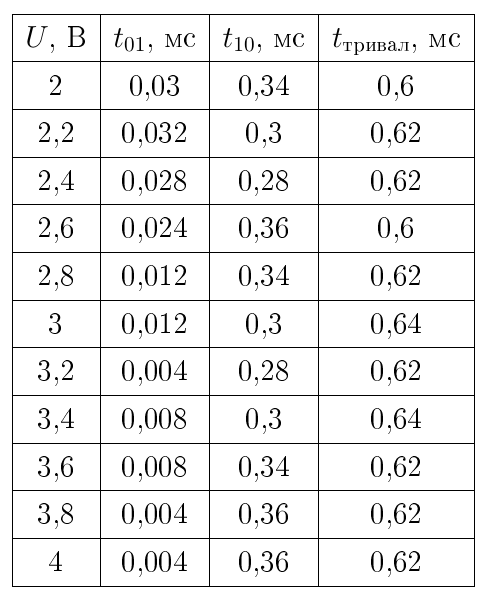
\includegraphics[width=0.7\linewidth]{t1.png}}

\label{ris2}
\end{figure}
 

\begin{itemize}


\item Піроелектричні приймачі - істинно пасивні пристрої.
Відповідно до природи піроелектричного ефекту для реєстрації
сигналу від приймача до нього не потрібно прикладати електричну напругу. В результаті відсутня складова шуму сигналу $1/f$, органічно властива мікроболометрів. Таким чином, теоретична межа NETD піроелектричних приймачів
у кілька разів нижче, ніж у мікроболометрів.
\item Технічний рівень матричних піроприймачів заснований також
на унікальній особливості піроприймачів – великий постійний час їх чутливих елементів (ЧЕ) (до 1–10 с).
\item Сигнал у піроелектричних приймачах має диференціальний характер. Оскільки піроприймачі реагують лише на зміну температури, вимоги до однорідності щодо чутливості окремих елементів матриці приймача знижуються у десятки разів. Завдяки цьому зменшується так званий фіксований просторовий або геометричний шум. Відповідно, при однакових значеннях NETD, що характеризують
тільки чутливість пікселів матриці, у системи на основі
піроелектриків спостерігається найкраще в порівнянні з мікроболометричними системами мінімальний дозвіл по різниці
температур реальних об'єктах (табл.3).
\item З тієї ж причини піроелектричні приймачі не чутливі до фонового випромінювання, яке для кімнатних температур
у робочому ІЧ-діапазоні дуже велике. На відміну від мікроболометрів на VOx і Si, для піроелектриків не потрібно спеціальної
обробки вихідного сигналу для віднімання фону та додаткового калібрування приймача для зміщення його робочої точки з метою підтримки прийнятного динамічного діапазону.
\item Існують дані, що показують, що матеріали, що відносяться
до класу піроелектриків, зберігають свої піроелектричні
властивості при впливах електромагнітних та радіаційних
випромінювань. Ця обставина може відіграти вирішальну роль
під час створення приладів для спецзастосування.
\item Нарешті, через те, що піроелектричний ефект залежить від поляризованості матеріалу, піроприймачі UFPA перспективні для створення нового покоління інтелектуальних сенсорів. Вони
можуть стати основою приймачів з перебудовуваною чутливістю, що виконують автоматичну корекцію неоднорідності чутливості, адаптацію до умов застосування та аналогову обробку сигналів.
\end{itemize}


Теоретична межа порогової чутливості ІЧ-приймального
пристрою визначається дробовим шумом потоку фонових фотонів,
що падають на фоточутливий елемент у межах його апертурного кута [4], і визначається співвідношенням:

\begin{equation}
NETD_r = \dfrac{NETD_r\cdot (\lambda)}{b\cdot Sin(\dfrac{\beta}{2})\cdot \sqrt{\tau_i}},
\end{equation}


де $NETD_r\cdot (\lambda)$
(l) – питома величина, яка залежить від спектрального
діапазону чутливості матриці (для $l$ = 10-12 мкм)\\
$NETD_r\cdot (\lambda)$ $\approx$ $10^{-7}$ К$\cdot$см$\cdot$с$^{-1/2}$),\\ 
b - крок матриці,\\ 
$\beta$ – кут поля зору матриці,\\ 
$t_i$ – час накопичення елементі матриці за кадр.\\ 
\begin{figure}[h!]
Таблиця 3. Реальні характеристики приймачів UFPA у порівнянні
з реальними характеристиками сегнетоелектричних та мікроболометричних детекторів [5]
\center{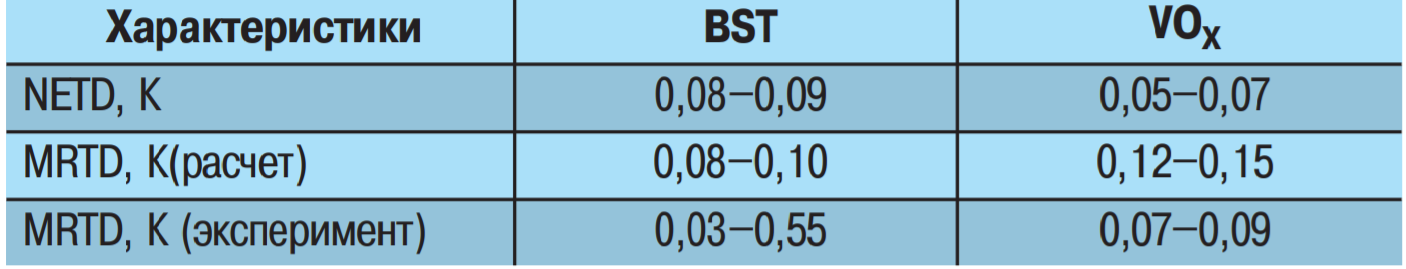
\includegraphics[width=0.9\linewidth]{t3.png}}

\label{ris2}
\end{figure}

Користуючись цим співвідношенням, можна порахувати, що за
b=15 мкм, $\beta$=27$^{\circ}$ (що відповідає об'єктиву F/1) і $t_i$ =1/30 з теоретичною межею еквівалентною шуму різниці температур для
мікроболометрів становить 0,37 мк. Врахування вищерозглянутих особливостей піроприймачів (відсутність дробового шуму, зменшення геометричного шуму, велика постійна часу накопичення
та ін) дозволяє оцінити їх теоретичну межу NETD, як мінімум, на порядок краще, ніж у мікроболометрів (тобто  0,04 мК). Вклад
власних шумів діелектричних втрат, властивих піроелектричним матеріалам, погіршує це значення в 2–3 (тобто. до значення  0,1 мК) [5].


\begin{figure}[h!]
\center{Таблиця 2. Неохолоджувані мікроболометричні матриці для спектрального діапазону 8-12 мкм}
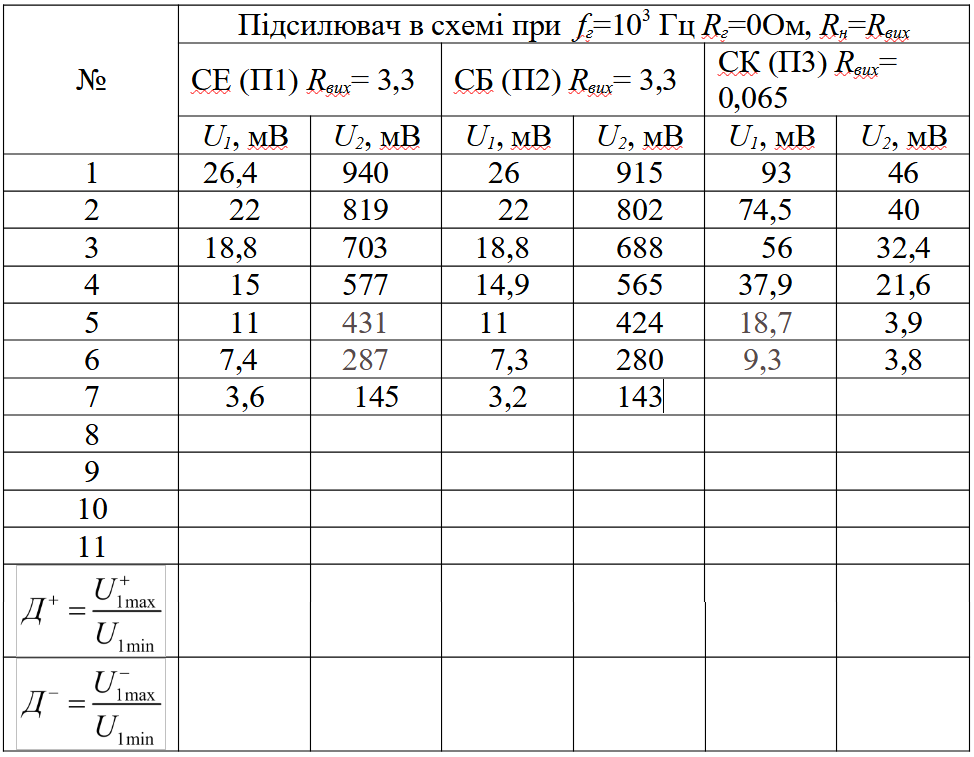
\includegraphics[width=0.9\linewidth]{t2.png}

\label{ris2}
\end{figure}

 %############################## 2 ########################## 
\chapter{ПРОБЛЕМИ СТВОРЕННЯ ПОЕП}\par
Широкому освоєнню випуску UFPA на основі піроелектриків перешкоджає комплекс проблем, що виникають під час створення матричних інтегральних теплових приймачів випромінювання. Це технологічність
конструкції та сумісність технології отримання теплочутливих детекторних матриць з базовими технологіями мікроелектроніки
Вирішення цих проблем йде декількома шляхами. Створення піроелектричних болометрів передбачає відпрацювання технологічних
процесів виготовлення багатоелементних піроприймачів UFPA на
основі сегнетоелектричної кераміки або матеріалів з низькими
температурами формування піроелектричних плівок та подальшої кристалізації піроелектриків у монолітній конструкції з
мультиплексор. Цікаві роботи в цьому напрямку проводять такі фірми як Raytheon Commercial Infrared, BAE Systems
(Avionics Group), NEC. У Росії аналогічні розробки невідомі.
Іншим напрямом створення ІЧ-приймачів на піроелектриках, в якому в Росії досягнуто помітних успіхів, є розробка піровідіконів (піриконів), що являють собою відікон

із суцільною або дрібноструктурною (мозаїчною) мішенню з піроелектрика (табл.4). Основна особливість піровидикону – відсутність
мультиплексора, роль якого виконує електронний пучок, що зчитує. Піровідикони відносяться до електровакуумних фоточутливих приладів ІЧ-діапазону (ІЧ ЕВФП).
\begin{figure}[h!]
\center{Таблиця 4. Порівняльні параметри піровидіконів
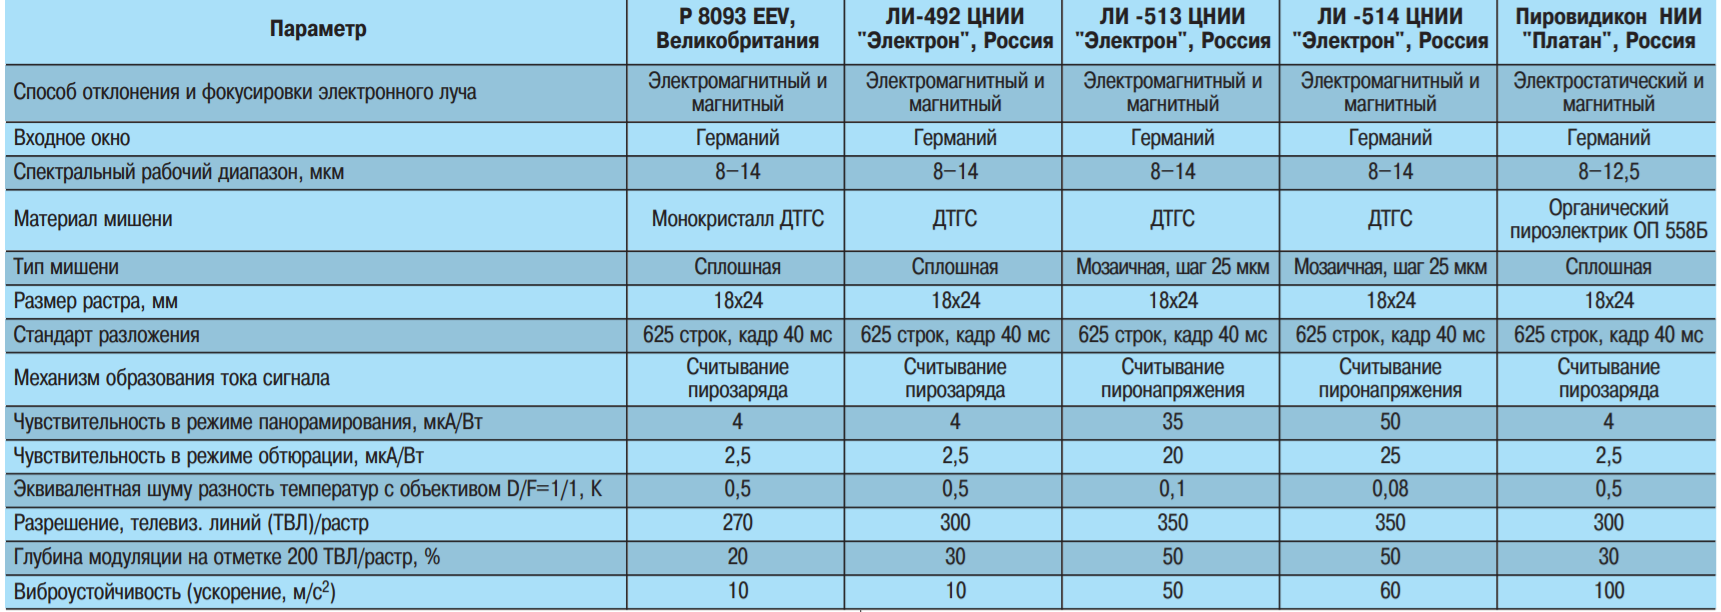
\includegraphics[width=0.9\linewidth]{t4.png}}

\label{ris2}
\end{figure}


Іншим прикладом конструкції багатоелементного ІЧ-приймача
служить піроелектричний електронно-оптичний перетворювач
(ПЕОП) [6]. Цей прилад може бути віднесений до нового класу приладів перетворення випромінювання діапазону 8-14 мкм для випромінювання видимого діапазону. Дія ПЕОП заснована на нетрадиційному для
цього виду фоточутливих приладів у фізичному принципі перетворення ІЧ-зображення у видиме – шляхом його попіксельної
дискретизації та модуляції однорідного потоку електронів матричним піроелектричним тепловим приймачем випромінювання.\par

Вплив ІЧ-випромінювання на чутливий елемент індукує в ньому електричний заряд, пропорційний потоку падаючого
випромінювання. Електричне поле наведеного заряду модулює потік
електронів, що проходять через отвори у ЧЕ. Для забезпечення
функціонування ПЕОП у ньому перед матрицею ЧЕ має бути у будь-який спосіб створено моноенергетичний потік електронів.
В іншому ПЕОП не відрізняється від традиційних ЕОП. Таким чином, ПЕОП є об'єднанням в одному приладі піроприймача та електронно-оптичного перетворювача, в якому
ІЧ-зображення перетворюється на видиме, що відображається на катодолюмінесцентному екрані ЕОП.

 %############################## 3 ########################## 
\chapter{КОНСТРУКТИВНО-ТЕХНОЛОГІЧНІ ОСОБЛИВОСТІ ПЕОП}\par



При опроміненні фотокатода відповідним джерелом підсвічування створюється однорідний просторовий потік фотоелектронів. Цей потік, проходячи через отвори піроелектричної мішені, модулюється відповідно до розподілу потенціалу на
поверхні піроелектричного шару, що виникає при проектуванні на ціль реєстрованого теплового випромінювання. Далі
модульований потік електронів, як у звичайному ЕОП, потрапляє
на пристрій реєстрації електронного зображення (катодолюмінесцентний екран), на якому візуально спостерігається розподіл теплового випромінювання, що реєструється (теплове поле об'єкта).
Для зручності спостерігача ПЕОП може додатково комплектуватися оптичним пристроєм перенесення та підсилювальним ЕОП.
На рис.4.1 наведено конструкцію зібраних макетних зразків.



\begin{figure}[h!]

\center{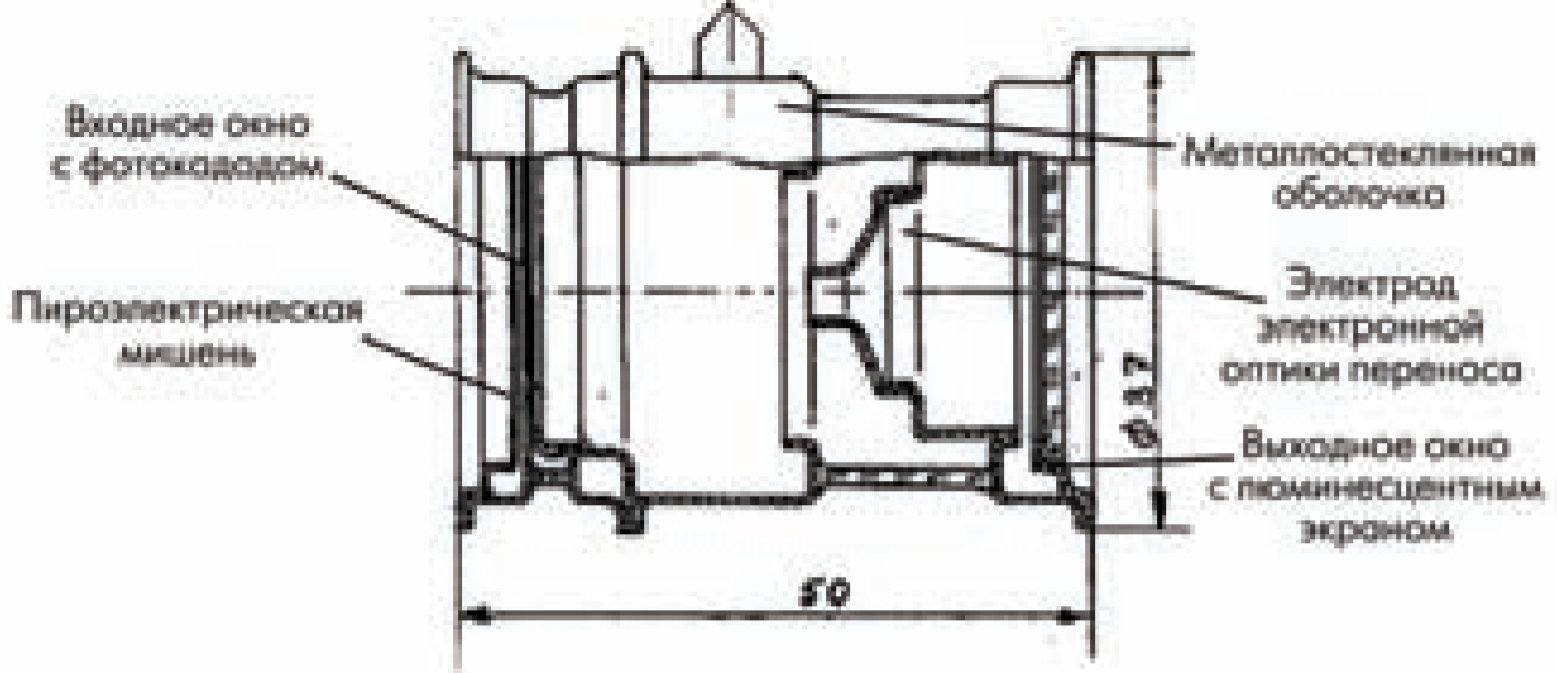
\includegraphics[width=0.7\linewidth]{r2.png}}
\caption{Конструкція виготовлених зразків ПЕОП}
\label{ris2}
\end{figure}

Основними елементами ПЕОП, що підлягають конструкторській та
технологічній розробці, є функціональні вузли: піроелектрична ціль, катод і вхідне вікно. Катодолюмінесцентний екран, оптика перенесення електронного зображення та підсилювач
на мікроканальній пластині повністю використовувалися з існуючих ЕОП. Основним функціональним вузлом ПЕОП, що фактично перетворює ЕОП звичайного діапазону в ЕОП діапазону 8-14 мкм,
є піроелектрична ціль.\par
Основне завдання мішені – перетворення двовимірного теплового зображення (8–14 мкм), спроектованого об'єктивом на поверхню мішені, на електричний двовимірний потенційний рельєф. Мета є і керуючим (модулюючим) електродом
для рівномірного електронного потоку, що проходить крізь неї. При
розробці конструкції такої мішені має бути забезпечене одночасне вирішення двох завдань: ефективне поглинання тепла та
забезпечення максимальної глибини модуляції електронного потоку,
проходить крізь ціль.\par
 Поставлене завдання вирішувалося в такий спосіб. Піроелектрична мета виконується з наскрізними отворами (1) для проходження електронного потоку. Піроелектричний
шар мішені (2) розділений наскрізними отворами на окремі
дискретні елементи. Ефективне поглинання тепла забезпечується металевими шарами поглинання (3, 5), нанесеними на несучу діелектричну плівку (4). Металевий електрод (3) одночасно виконує функцію електрода, що управляє. Поглинене
тепло перетворюється за допомогою піроелектричного шару на електричний потенційний рельєф на поверхні мішені, що повторює
картину розподілу тепла за перерізом теплового потоку. Ефективність теплового перетворення залежить від вибору
матеріалу піроелектрика. Глибина модуляції, що проходить крізь
Мета електронного потоку визначається значенням електричного
потенційного рельєфу та геометрією сітчастого електрода.\par 
Один із основних елементів
ПЕОП – джерело електронного
потоку, який повинен створювати просторово-однорідний потік електронів, що використовується для перетворення просторового розподілу
потенціалів на піроелектричній мішені у видиме зображення на катодолюмінесцентному
екран. Джерело електронів може виконуватися не обов'язково за допомогою фотокатода, а може бути будь-якого типу. Важлива вимога до джерела електронів – спосіб збудження електронного потоку та склад активної речовини джерела не повинні впливати на працездатність піроелектричної
цілі, в тому числі і в процесі експлуатації ПЕОП. Всім цим
вимогам задовольняють кілька типів джерел електронів: фотокатод як елемент, традиційний для ЕОП, та автоемісійний катод як елемент, який може бути використаний
в перспективі. Зважаючи на те, що як матеріал фотокатода
був обраний паладій, що працює в короткохвильовій частині УФ спектру, як вхідне вікно для макетних зразків приладу
використовувалися кристали фтористого магнію, прозорого в УФчастині спектру.






















\begin{thebibliography}{9}
\bibitem{lit1} Филачев А.М., Пономаренко В.П., Таубкин И.И., Ушакова М.Б.
Инфракрасные матрицы и тенденции их развития.—Труды XVIII международной конференции по фотоэлектронике и приборам ночного видения.—М., 2004.
\bibitem{lit2} Певцов Е.Ф. Матричные ИК приемники и портативные системы
визуализации инфракрасного излучения. Труды XVIII международной конференции по фотоэлектронике и приборам ночного видения. М., 2004.
\bibitem{lit3} https://nplus1.ru/news/2017/03/09/information-density-record
\bibitem{lit4} II International Scientific Practical Conference of graduate and postgraduate students,
lecturers «APPLIED ISSUES OF EXACT SCIENCES»
19-20 October 2018, Armavir(http://amti.esrae.ru/pdf/2018/3(1)/197.pdf)
\bibitem{lit5} https://compress.ru/article.aspx?id=10717part=31ext1
\bibitem{lit6} https://compress.ru/article.aspx?id=10717
\bibitem{lit7} https://aip.scitation.org/doi/10.1063/1.1953879
\bibitem{lit8} \href{https://www.researchgate.net/publication/224354512_Heat_Assisted_Magnetic_Recording}{Heat Assisted Magnetic Recording}
\bibitem{lit9}
\bibitem{lit10}
\end{thebibliography}
\end{document}
